\documentclass{article} % say
\usepackage{tikz}
\usetikzlibrary{arrows,  % 箭头的library
  decorations.pathmorphing, % snake-line
  backgrounds,              % 背景
  positioning,              % 相对地放置节点
  fit,                      % 计算size的东西
  petri}
\begin{document}

% ===================================================
% 以下三段代码具有相同的效果
\begin{tikzpicture}
\path ( 0,2) node [shape=circle,draw] {}
( 0,1) node [shape=circle,draw] {}
( 0,0) node [shape=circle,draw] {}
( 1,1) node [shape=rectangle,draw] {}
(-1,1) node [shape=rectangle,draw] {};
\end{tikzpicture}

\begin{tikzpicture}
\path node at ( 0,2) [shape=circle,draw] {}
node at ( 0,1) [shape=circle,draw] {}
node at ( 0,0) [shape=circle,draw] {}
node at ( 1,1) [shape=rectangle,draw] {}
node at (-1,1) [shape=rectangle,draw] {};
\end{tikzpicture}

\begin{tikzpicture}
\node at ( 0,2) [circle,draw] {};
\node at ( 0,1) [circle,draw] {};
\node at ( 0,0) [circle,draw] {};
\node at ( 1,1) [rectangle,draw] {};
\node at (-1,1) [rectangle,draw] {};
\end{tikzpicture}

% =============================================================

% 这种node的方式同样支持各种自定义style
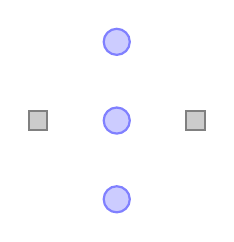
\begin{tikzpicture}[thick]
\node at ( 0,2) [circle,draw=blue!50,fill=blue!20] {};
\node at ( 0,1) [circle,draw=blue!50,fill=blue!20] {};
\node at ( 0,0) [circle,draw=blue!50,fill=blue!20] {};
\node at ( 1,1) [rectangle,draw=black!50,fill=black!20] {};
\node at (-1,1) [rectangle,draw=black!50,fill=black!20] {};
\end{tikzpicture}

% 整体的一个图片文档的思路,下面将会重点对其进行介绍。
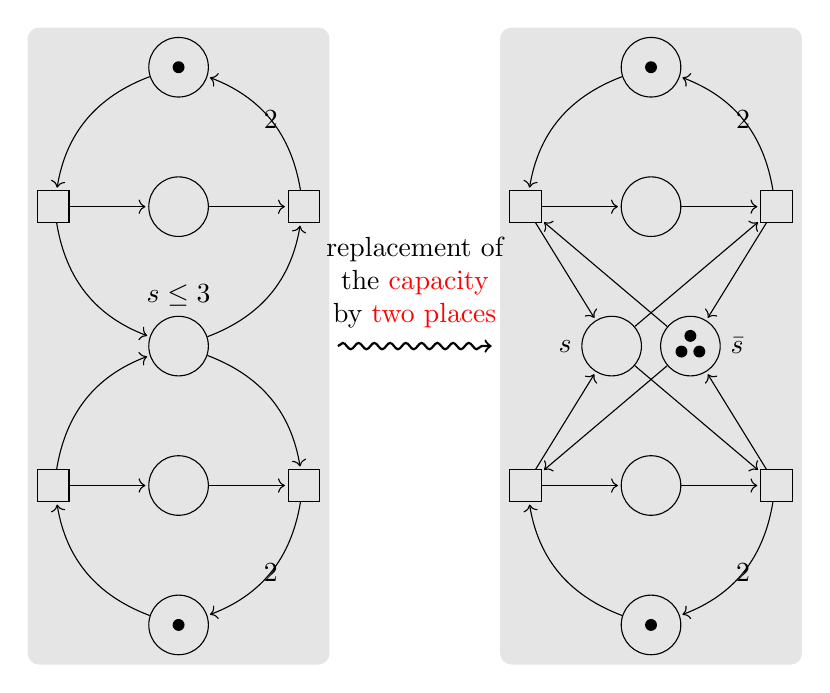
\begin{tikzpicture}style[node distance=1.3cm,on grid,>={Stealth[round]},bend angle=45,auto,
  % 定义了全局的style特点:节点间距离是1.3cm,on grid 是一个特殊的模式,
  % bend angle是用来形容曲线拐角的角度的

  % 以下定义了几个主要的style:
  {every place}/.style={minimumsize=6mm,thick,draw=blue!75,fill=blue!20},

  {every transition}/.style={thick,draw=black!75,fill=black!20},

  {red place}/.style= {place,draw=red!75,fill=red!20},

  {every label}/.style= {red}]

  \usetikzlibrary {arrows.meta,petri,positioning} %引用了使用的library。


  \node [place,tokens=1] (w1) {};
  \node [place] (c1) [below=of w1] {};
  \node [place] (s) [below=of c1,label=above:$s\le 3$] {};
  \node [place] (c2) [below=of s] {};
  \node [place,tokens=1] (w2) [below=of c2] {};
  \node [transition] (e1) [left=of c1] {}
  edge [pre,bend left] (w1)    % 代表style是pre格式,且从本节点(e1)
                               % 指向其他节点

  edge [post,bend right] (s)
  edge [post] (c1);
  

  \node [transition] (e2) [left=of c2] {}

  edge [pre,bend right] (w2)

  edge [post,bend left] (s)

  edge [post] (c2);

  \node [transition] (l1) [right=of c1] {}

  edge [pre] (c1)

  edge [pre,bend left] (s)

  edge [post,bend right] node[swap] {2} (w1);

  \node [transition] (l2) [right=of c2] {}

  edge [pre] (c2)

  edge [pre,bend right] (s)

  edge [post,bend left] node {2} (w2);

  \usetikzlibrary {arrows.meta,petri,positioning}

  \begin{scope}[xshift=6cm]  % 进行一个屏蔽,这个子模块遵从特殊的形式,
                             % 其形式为xshift=6cm

    \node [place,tokens=1] (w1') {};

    \node [place] (c1') [below=of w1'] {};

    \node [place] (s1') [below=of c1',xshift=-5mm,label=left:$s$] {};
    % $$指的是通过latex代码来写处对这个node的标注的内容

    \node [place,tokens=3] (s2') [below=of c1',xshift=5mm,label=right:$\bar s$] {};

    \node [place] (c2') [below=of s1',xshift=5mm] {};

    \node [place,tokens=1] (w2') [below=of c2'] {};

    \node [transition] (e1') [left=of c1'] {}

    edge [pre,bend left] (w1')

    edge [post] (s1')

    edge [pre] (s2')

    edge [post] (c1');

    \node [transition] (e2') [left=of c2'] {}

    edge [pre,bend right] (w2')

    edge [post] (s1')

    edge [pre] (s2')

    edge [post] (c2');

    \node [transition] (l1') [right=of c1'] {}

    edge [pre] (c1')

    edge [pre] (s1')

    edge [post] (s2')

    edge [post,bend right] node[swap] {2} (w1');

    \node [transition] (l2') [right=of c2'] {}

    edge [pre] (c2')

    edge [pre] (s1')

    edge [post] (s2')

    edge [post,bend left] node {2} (w2');

  \end{scope}


  \begin{scope}[on background layer]

    \node (r1) [fill=black!10,rounded corners,fit=(w1)(w2)(e1)(e2)(l1)(l2)] {};

    \node (r2) [fill=black!10,rounded corners,fit=(w1')(w2')(e1')(e2')(l1')(l2')] {};

  \end{scope}


  \draw [shorten >=1mm,-to,thick,decorate,decoration={snake,amplitude=.4mm,segment length=2mm, pre=moveto,pre length=1mm,post length=2mm}]

  (r1) -- (r2) node [above=1mm,midway,text width=3cm,align=center]{replacement of the \textcolor{red}{capacity} by \textcolor{red}{two places}};

\end{tikzpicture}








\begin{tikzpicture}
\draw (0,0) -- (1,1);
\end{tikzpicture}
\end{document}













%%% Local Variables:
%%% mode: latex
%%% TeX-master: t
%%% End:
